\chapter{Fonctions du 3\up{ème} degré}

\section{Généralités et définitions}

\subsection{Définition d'une fonction du 3\up{ème} degré}

\begin{defin}[Fonction du 3\up{ème} degré]
	Les fonctions définies sur $\mathbb{R}$ par :

	\[
		x \longmapsto ax^{3}\qquad\text{ou}\qquad x \longmapsto ax^{3}+b
	\]

	\ldots sont des \textbf{fonctions du $3$\up{ème} degré}.

	Les coefficients $a$ et $b$ sont des réels donnés avec $a \neq 0$.

	\begin{itemize}
		\item \textbf{Exemples}
		      \begin{itemize}
			      \item $f(x)=4x^{\textcolor{red}{3}}+1$
			      \item $g(x)=x^{\textcolor{red}{3}}-2$
			      \item $h(x)=1+x^{2}-2x^{\textcolor{red}{3}}$
		      \end{itemize}
		\item \textbf{Contre-exemples}
		      \begin{itemize}
			      \item $m(x)=-x+4$\qquad\ldots est une fonction affine
			      \item $n(x)=2x^{5}-x^{3}+5x-1$\qquad\ldots est une fonction du 5\up{ème} degré
		      \end{itemize}
	\end{itemize}
\end{defin}

\subsection{Représentation graphique et sens de variation}

\begin{prop}[Variations des fonctions $x \mapsto ax^3+b$]
	Soit $f$ une fonction du $3$\up{ème} degré, telle que :
	\[
		f(x)=ax^{3}+b
	\]

	\begin{itemize}
		\item Si $a>0$ : $f$ est strictement \textbf{croissante} sur $\mathbb{R}$.
		\item Si $a<0$ : $f$ est strictement \textbf{décroissante} sur $\mathbb{R}$.
	\end{itemize}

	\begin{center}
		\begin{tikzpicture}[scale=0.6, >=Stealth]
			\begin{scope}
				\def\xmin{-6.5}\def\xmax{4.5}\def\ymin{-4.8}\def\ymax{5.5}
				\clip (\xmin, \ymin) rectangle (\xmax, \ymax);
				\draw[->, thick] (\xmin, 0) -- (\xmax, 0) node[above left] {$x$};
				\draw[->, thick] (0, \ymin) -- (0, \ymax) node[below right] {$y$};
				\foreach \x in {-6,-5,-4,-3,-2,-1,1,2,3,4} \draw (\x, 0.1) -- (\x, -0.1) node[below, font=\footnotesize] {$\x$};
				\foreach \y in {-4,-3,-2,-1,1,2,3,4,5} \draw (0.1, \y) -- (-0.1, \y) node[left, font=\footnotesize] {$\y$};
				\draw[domain=-2.8:2.8, smooth, very thick, dashed, green!50!black] plot (\x, {0.25*\x^3});
				\draw[domain=-2.8:2.8, smooth, very thick, red!60!black] plot (\x, {-0.25*\x^3});
				\node[left] at (-2.9, 0.8) {$f(x)=ax^3$};
				\node[red!60!black] at (-3.7, 4.5) {$a < 0$};
				\node[green!50!black] at (3.5, 4.5) {$a > 0$};
			\end{scope}
			\begin{scope}[xshift=13cm]
				\def\xmin{-7.5}\def\xmax{4.5}\def\ymin{-4.8}\def\ymax{5.5}
				\clip (\xmin, \ymin) rectangle (\xmax, \ymax);
				\draw[->, thick] (\xmin, 0) -- (\xmax, 0) node[above left] {$x$};
				\draw[->, thick] (0, \ymin) -- (0, \ymax) node[below right] {$y$};
				\foreach \x in {-7,-6,-5,-4,-3,-2,-1,1,2,3,4} \draw (\x, 0.1) -- (\x, -0.1) node[below, font=\footnotesize] {$\x$};
				\foreach \y in {-4,-3,-2,-1,1,2,3,4,5} \draw (0.1, \y) -- (-0.1, \y) node[left, font=\footnotesize] {$\y$};
				\draw[domain=-3.1:2.5, smooth, very thick, dashed, green!50!black] plot (\x, {0.25*\x^3 + 2});
				\draw[domain=-3.5:3.1, smooth, very thick, red!60!black] plot (\x, {-0.25*\x^3 - 1});
				\node[left] at (-2.9, 0.8) {$f(x)=ax^3+b$};
				\node[red!60!black] at (-3.8, 4.5) {$a < 0$};
				\node[green!50!black] at (3.1, 4.5) {$a > 0$};
			\end{scope}
		\end{tikzpicture}
	\end{center}
\end{prop}

\section{Forme factorisée, racines et étude de signe}

\subsection{Forme factorisée et racines}

\begin{ex}[Passage de la forme factorisée à la forme développée]
	La fonction $f$ définie par $f(x)=5(x-4)(x-1)(x+3)$ est une fonction du $3$\up{ème} degré sous sa forme \textbf{factorisée}.

	Si on développe l'expression de $f$, on obtient bien l'expression d'un polynôme du $3$\up{ème} degré :
	\[
		\begin{array}{rcl}
			f(x) & = & 5(x-4)\underbrace{(x-1)(x+3)}   \\
			     & = & 5\underbrace{(x-4)(x^2+2x-3)}   \\
			     & = & \underbrace{5(x^3-2x^2-11x+12)} \\
			     & = & 5x^{3}-10x^{2}-55x+60
		\end{array}
	\]
\end{ex}

\begin{defin}[Forme factorisée]
	Les fonctions définies sur $\mathbb{R}$ par :
	\[
		f(x)=a(x-x_{1})(x-x_{2})(x-x_{3})
	\]

	\ldots sont des fonctions du $3$\up{ème} degré sous \textbf{forme factorisée}.

	Les nombres $a$, $x_{1}$, $x_{2}$ et $x_{3}$ sont des réels avec $a \neq 0$.
\end{defin}

\begin{prop}[Racines et intersection avec l'axe des abscisses]
	Soit la fonction $f$ définie sur $\mathbb{R}$ par $f(x)=a(x-x_{1})(x-x_{2})(x-x_{3})$.

	L'équation $f(x)=0$ possède trois solutions (éventuellement égales) :
	\[
		S=\{x_{1} \,;\, x_{2} \,;\, x_{3}\}
	\]

	Ces solutions sont appelées les \textbf{racines} de la fonction $f$.

	Graphiquement, dire que $x_1$, $x_2$ et $x_3$ sont les racines de $f$ signifie que la courbe représentative $\mathcal{C}_f$ coupe l'axe des abscisses en trois points de coordonnées respectives $(x_{1}\,;\,0)$, $(x_{2}\,;\,0)$ et $(x_{3}\,;\,0)$.

	\begin{center}
		\begin{tikzpicture}[>=Stealth, y=8mm]
			\def\xmin{-4.5}\def\xmax{5.5}\def\ymin{-3.5}\def\ymax{3.5}
			\clip (\xmin, \ymin) rectangle (\xmax, \ymax);
			\draw[step=1, gray!40] (\xmin, \ymin) grid (\xmax, \ymax);
			\draw[->, thick] (\xmin, 0) -- (\xmax, 0) node[above left] {$x$};
			\draw[->, thick] (0, \ymin) -- (0, \ymax) node[below right] {$y$};
			\node[red, fill=white] at (5.1, 2) {$\mathcal{C}_f$};
			\draw[domain=\xmin:\xmax, smooth, ultra thick, red] plot (\x, {0.1*(\x+3)*(\x-1)*(\x-4)});
			\foreach \x in {-3,1,4} \filldraw (\x, 0) circle (2pt);
			\node[above left] at (-3, 0) {$x_1$};
			\node[above right] at (1, 0) {$x_2$};
			\node[above left] at (4, 0) {$x_3$};
		\end{tikzpicture}
	\end{center}
\end{prop}

\begin{ex}[Vérification des racines et représentation graphique]
	Soit $f$ la fonction définie sur $\mathbb{R}$ par :
	\[
		f(x) = 5(x-4)(x-1)(x+3) \quad = 5x^{3}-10x^{2}-55x+60
	\]

	On peut vérifier par le calcul que $-3$, $1$ et $4$ sont des racines de $f$ :
	\begin{itemize}
		\item $f(\textcolor{blue}{-3}) = 5{\times \textcolor{blue}{(-3)}}^{3}-10 \times \textcolor{blue}{(-3)}^{2}-55 \times \textcolor{blue}{(-3)}+60 = -135-90+165+60 = 0$
		\item $f(\textcolor{red}{1}) = 5\times \textcolor{red}{1}^{3}-10 \times \textcolor{red}{1}^{2}-55 \times \textcolor{red}{1}+60 = 5-10-55+60 = 0$
		\item $f(\textcolor{vert}{4}) = 5\times \textcolor{vert}{4}^{3}-10 \times \textcolor{vert}{4}^{2}-55 \times \textcolor{vert}{4}+60 = 320-160-220+60 = 0$
	\end{itemize}

	Les nombres $-3$, $1$ et $4$ sont donc les racines de $f$.

	Sa courbe représentative coupe l'axe des abscisses en ces trois mêmes valeurs :

	\begin{center}
		\begin{tikzpicture}[>=Stealth,y=0.25mm]
			\def\xmin{-4.2}\def\xmax{5.5}\def\ymin{-75}\def\ymax{115}
			\clip (\xmin, \ymin) rectangle (\xmax, \ymax);
			\draw[step=1, ystep=20, gray!30] (\xmin, \ymin) grid (\xmax, \ymax);
			\draw[->, thick] (\xmin, 0) -- (\xmax, 0) node[above left] {$x$};
			\draw[->, thick] (0, \ymin) -- (0, \ymax) node[below right] {$y$};
			\node[left] at (0, 60) {$60$};
			\draw[domain=\xmin:\xmax, smooth, ultra thick, red] plot (\x, {5*(\x+3)*(\x-1)*(\x-4)});
			\foreach \x in {-3,1,4} \filldraw (\x, 0) circle (2pt);
			\filldraw (0, 60) circle (2pt);
			\node[above left] at (-3, 0) {$-3$};
			\node[above right] at (1, 0) {$1$};
			\node[above right] at (4, 0) {$4$};
			\node[above left, red] at (-2, 90) {$\mathcal{C}_f$};
		\end{tikzpicture}
	\end{center}
\end{ex}

\subsection{Variations générales d'un polynôme du 3\up{ème} degré}

\begin{prop}[Allure générale et extremums]
	Soit $f$ une fonction du 3\up{ème} degré définie sur $\mathbb{R}$.

	Lorsque la fonction $f$ admet deux extremums locaux distincts atteints en $\alpha$ et $\beta$ (avec $\alpha < \beta$), ses variations sont données par les tableaux ci-dessous :

	\begin{center}
		\begin{tabular}{cc}
			\textbf{Cas $a > 0$} & \textbf{Cas $a < 0$} \\[0.5em]
			\begin{tikzpicture}[scale=0.8]
				\tikzset{arrow style/.style={->, >=Triangle, thick}}
				\tkzTabInit[lgt=1.5, espcl=1.8]{$x$ / 0.8, $f$ / 1.8}{$-\infty$, $\alpha$, $\beta$, $+\infty$}
				\tkzTabVar{-/ , +/ $f(\alpha)$, -/ $f(\beta)$, +/ }
			\end{tikzpicture}
			                     &
			\begin{tikzpicture}[scale=0.8]
				\tikzset{arrow style/.style={->, >=Triangle, thick}}
				\tkzTabInit[lgt=1.5, espcl=1.8]{$x$ / 0.8, $f$ / 1.8}{$-\infty$, $\alpha$, $\beta$, $+\infty$}
				\tkzTabVar{+/ , -/ $f(\alpha)$, +/ $f(\beta)$, -/ }
			\end{tikzpicture}
		\end{tabular}
	\end{center}

	\begin{remarque}
		Pour les fonctions particulières de la forme $f(x) = ax^3 + b$, la fonction n'admet pas deux extremums locaux et est strictement monotone sur $\mathbb{R}$ (strictement croissante si $a>0$, strictement décroissante si $a<0$).
	\end{remarque}
\end{prop}

\subsection{Méthode : Étude du signe}

\begin{methode}[Étude du signe d'une fonction du $3$\up{ème} degré]
	Étudions le signe de la fonction $f$ définie sur $\mathbb{R}$ par $\quad f(x)=2(x+1)(x-2)(x-5)$

	Le signe de $2(x+1)(x-2)(x-5)$ dépend du signe des facteurs $(x+1)$, $(x-2)$ et $(x-5)$ et du signe de $a$.

	On étudie ainsi le signe de chaque facteur et on présente les résultats dans un tableau de signes.
	\begin{itemize}
		\item $x+1=0 \iff x_1=-1$
		\item $x-2=0 \iff x_2=2$
		\item $x-5=0 \iff x_3=5$
	\end{itemize}

	Les nombres $-1$, $2$ et $5$ sont donc les racines de $f$.

	En appliquant la règle des signes dans le tableau ci-dessous, on en déduit le signe de $f(x)$ :

	\begin{center}
		\begin{tikzpicture}
			\tkzTabInit[lgt=4.5, espcl=2]{$x$ / 0.7, $a=2$/0.7, $x+1$ / 0.7, $x-2$ / 0.7, $x-5$ / 0.7, $f(x)=2(x+1)(x-2)(x-5)$ / 0.7}{$-\infty$, $-1$, $2$, $5$, $+\infty$}
			\tkzTabLine{ , +, t, +, t, +, t, + }
			\tkzTabLine{ , -, z, +, t, +, t, + }
			\tkzTabLine{ , -, t, -, z, +, t, + }
			\tkzTabLine{ , -, t, -, t, -, z, + }
			\tkzTabLine{ , -, z, +, z, -, z, + }
		\end{tikzpicture}
	\end{center}

	On en déduit que :
	\begin{itemize}
		\item $f(x) \ge 0$ pour $x \in \intff{-1}{2} \cup \intfo{5}{+\infty}$
		\item $f(x) \le 0$ pour $x \in \intof{-\infty}{-1} \cup \intff{2}{5}$
	\end{itemize}

	\begin{center}
		\begin{tikzpicture}[x=15mm, y=1.25mm, >=Stealth]
			\def\xmin{-2.5}\def\xmax{6.5}\def\ymin{-24}\def\ymax{24}
			\clip (\xmin, \ymin) rectangle (\xmax, \ymax);
			\draw[ystep=5, gray!25] (\xmin, \ymin) grid (\xmax, \ymax);
			\draw[->, thick] (\xmin, 0) -- (\xmax, 0) node[above left] {$x$};
			\draw[->, thick] (0, \ymin) -- (0, \ymax) node[below left] {$y$};
			\node[fill=white] at (5, 20) {$\mathcal{C}_f$};
			\draw[domain=-3.3:-1, smooth, ultra thick, rouge, dashed] plot (\x, {2*(\x+1)*(\x-2)*(\x-5)});
			\draw[domain=-1:2, smooth, ultra thick, vert] plot (\x, {2*(\x+1)*(\x-2)*(\x-5)});
			\draw[domain=2:5, smooth, ultra thick, rouge,dashed] plot (\x, {2*(\x+1)*(\x-2)*(\x-5)});
			\draw[domain=5:6.8, smooth, ultra thick, vert] plot (\x, {2*(\x+1)*(\x-2)*(\x-5)});
			\foreach \x/\label/\pos in {-1/-1/above left, 2/2/above right, 5/5/above left} { \filldraw (\x,0) circle (2pt); \node[\pos] at (\x, 0) {$\label$}; }
			\node[rouge, font=\Large] at (-1.7, -13) {$-$};
			\node[vert, font=\Large] at (0.6, 15) {$+$};
			\node[rouge, font=\Large] at (3.5, -13) {$-$};
			\node[vert, font=\Large] at (5.7, 12) {$+$};
		\end{tikzpicture}
	\end{center}
\end{methode}

\section{Équations du type $x^{3}=c$}

\subsection{Propriétés}

\begin{prop}[Résolution de l'équation $x^3=c$]
	L'équation $x^{3}=c$, avec $c$ positif, possède une \textbf{unique} solution $\sqrt[3]{c}$.

	Cette solution peut également se calculer à l'aide de $\sqrt[3]{c} = c^{\frac{1}{3}}$.
	\[
		x^3=c \iff x=\sqrt[3]{c}=c^{\frac{1}{3}}
	\]
\end{prop}

\subsection{Méthodes de résolution}

\begin{methode}[Résoudre une équation du type $x^3=c$]
	\nline
	\begin{itemize}
		\item \textbf{Résoudre dans $\mathbb{R}$ l'équation $x^{3}=27$ :}

		      On cherche le nombre qui, élevé au cube, donne $27$.

		      Ce nombre est égal à la \textbf{racine cubique} de $27$, soit $x=\sqrt[3]{27}=27^{\frac{1}{3}}=3$.

		      \textbf{Vérification :}

		      Comme $3^{3} = 27$, $3$ est bien une solution. C'est la seule et unique solution de l'équation.

		\item \textbf{Résoudre dans $\mathbb{R}$ l'équation $2x^{3}-6=16$ :}

		      Pour résoudre cette équation, il faut se ramener à la forme $x^3=c$ :
		      \[
			      \begin{array}{rrcl}
				           & 2x^{3}-6 & = & 16                                           \\
				      \iff & 2x^{3}   & = & 22                                           \\
				      \iff & x^{3}    & = & 11                                           \\
				      \iff & x        & = & \sqrt[3]{11}=11^{\frac{1}{3}}\approx 2,22398
			      \end{array}
		      \]
	\end{itemize}
\end{methode}
